\newpage
\section{Revisão da Teoria}

\subsection{Geração do código bi-fase}
	Em sistemas de telecomunicação a codificação bi-fase consiste em um código de linha onde cada bit é representado por uma transição de nível lógico, isto é, para representar o bit 1, é necessário uma transição do nível lógico alto para o nível lógico baixo e para representar o bit 0, uma transição do nível lógico baixo para o nível lógico alto. A Figura \ref{fig:bi} mostra graficamente a representação de um sinal de dados NRZ com a codificação bi-fase.
	
	A regra para se gerar o sinal com codificação é: o primeiro meio período de bit possui o mesmo nível lógico do dado a ser transmitido, já a segunda metade do período de bit é o nível lógico inverso.
		
	Essa regra faz com que o nível DC do sinal seja constante para todos períodos de bit, porém, o mesmo pode ser recuperado na recepção através da média dos dois níveis recebidos.
	
	\begin{figure}[H]
		\centering
		\caption{Representação gráfica para a codificação bi-fase.}
		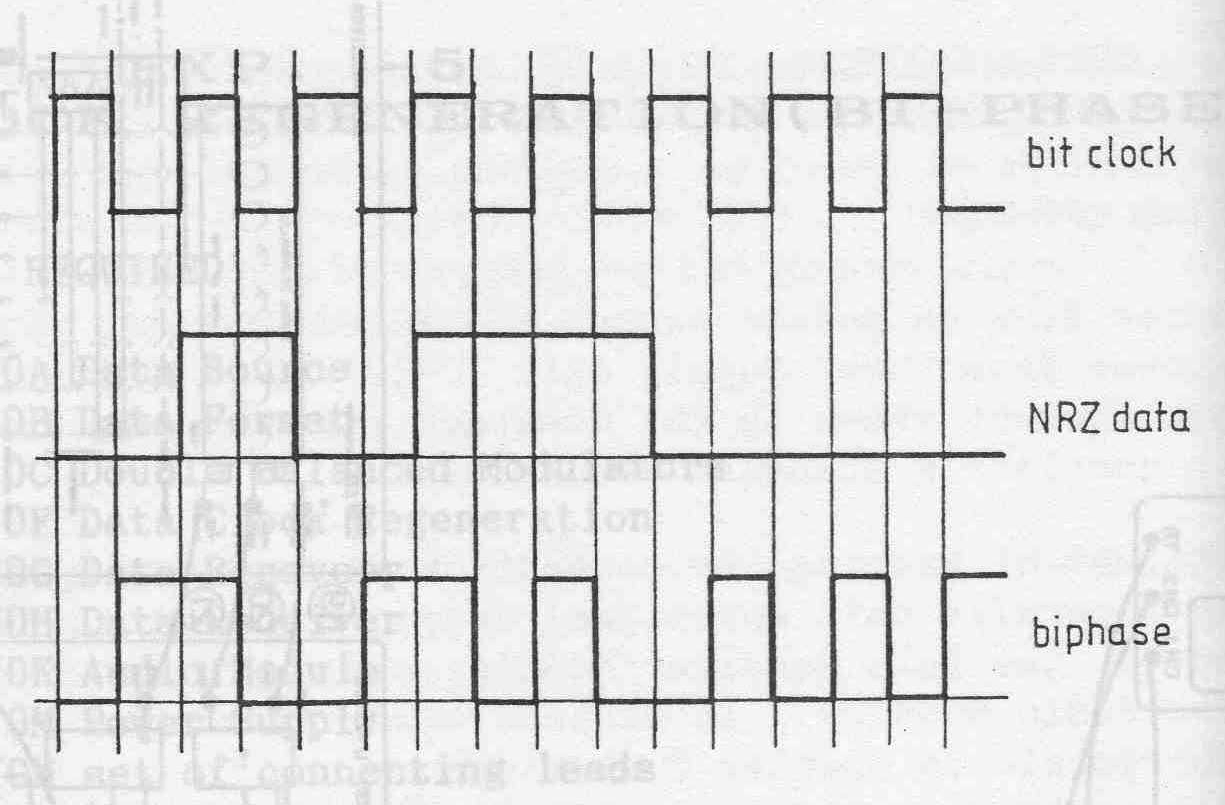
\includegraphics[scale=0.3]{bi}
			
		\small Fonte: Jacob, J. L., Roteiro de laboratório, 2017.
		\label{fig:bi}
	\end{figure}
		
	Uma das vantagens da codificação bi-fase é que o clock de bit acompanha o sinal transmitido, podendo ser regenerado no receptor, evitando a necessidade de se transmitir um sinal adicional com o clock.
	
	Outra vantagem é a possibilidade do nível DC igual a zero para um período de bit, pois alguns canais não permitem a transmissão com um nível DC.
	
	
\subsection{Regeneração do clock}

	A regeneração do clock emprega um comparador de frequência e fase, o qual tem a função de sincronizar os dados com o clock dos pulsos extraídos do sinal bi-fásico. Para verificar se os clocks de bits originais e os regenerados estão fora de fase, o comparador busca uma transição do clock no dobro do período do clock dos pulsos extraídos. Caso não haja essa transição, o comparador reverte a fase do clock regenerador, causando a regeneração do clock correspondente ao original.
	
	Assim, os dados podem ser recuperados de acordo com as transições apresentadas no período de cada pulso de clock.
	
\subsection{Recuperação dos dados}

	Os dados recuperados no receptor necessitam de limpeza, pois possuem picos no sinal NRZ recuperado. Sendo assim, a técnica \textit{integrate and dump} pode ser aplicada para recuperar o sinal NRZ limpo.
	
	Essa técnica consiste em integrar os dados NRZ e, após 1 período de bit amostrar o sinal, passando por um decisor que dirá se o respectivo bit é 1 ou 0. Ao termino de cada período de bit, o integrador deve ser zerado.
	
	Uma das consequências de se utilizar essa técnica é o atraso de 1 período de bit na recepção, devido ao tempo necessário para se integrar e amostrar o sinal.
	
	A Figura \ref{fig:integrate} demonstra a operação da técnica \textit{integrate and dump}.
	
		\begin{figure}[H]
			\centering
			\caption{Técnica \textit{integrate and dump}.}
			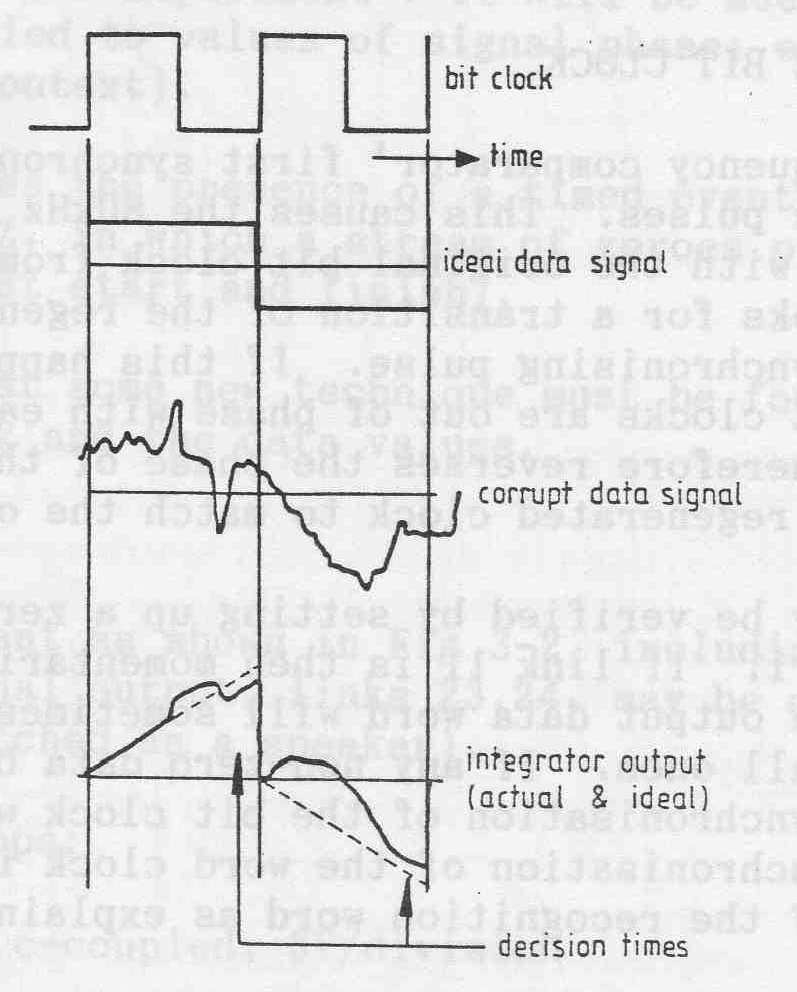
\includegraphics[scale=0.3]{integrate}
			
			\small Fonte: Jacob, J. L., Roteiro de laboratório, 2017.
			\label{fig:integrate}
		\end{figure}